% !TEX root = template.tex

\theoremstyle{definition}
\newtheorem{definition}{Definition}[section]

\theoremstyle{definition}
\newtheorem{optimization}{Optimization Problem}

\section{Introduction}

Here goes the introduction. We also cite the nice book by \citet{Pinedo:2012}.
This might be a book with interesting topics, but concurrent time-stamping has also been addressed before~\cite{Dolev97}.
In this work, \citet{Dolev97} presented the first bounded implementation of a concurrent time-stamp system.

\section{Scheduling Algorithm}

\citet*{Chen2017} view a data analytic \emph{job} simply as a number of \emph{tasks} that comprise it. These tasks are further separated into consecutive \emph{stages}, where the future stages depend on the results of the past stages. In other words, the tasks from a single stage must wait for the tasks from all the previous stages to complete. On the contrary, within a single stage the tasks are \emph{independent} of each other and therefore could be executed in parallel.

\citet{Chen2017} further describe a geographically distributed datacenter as a group of independent datacenters connected by a network. Each single datacenter from this group contains several \emph{computing slots} which are capable of executing tasks. Furthermore, the network that connects the pairs of datacenters is expected to have significantly \emph{lower bandwidth} than the local network inside each individual datacenter. This means that transferring large amounts of data between different datacenters takes a lot of time. Finally, in order to execute a task, it must be provided with a computing slot and the necessary input data. The input data for every task is also hosted by some datacenter(s). If it so happens that a task is assigned to a datacenter that does not hold the entire input data for that task, the missing parts will be transferred across the inter-datacenter network.

\subsection{Formal Definitions}

\citet*{Chen2017} define \(\mathcal{D} = \left\{1, 2, \dots, J\right\}\) to be the set whose elements are individual datacenters and the entire set itself represents one large geographically distributed datacenter. Each individual datacenter \(j\) has a limited number of computing slots denoted by \(a_j\). Furthermore, the set of analytic jobs is defined as \(\mathcal{K} = \left\{1, 2, \dots, K\right\}\). Each of the jobs \(k\) consists of a single stage which itself is a set of independent tasks \(\mathcal{T}_k=\left\{1, 2, \dots, n_k\right\}\).

In the proposed theoretical model the time it takes to complete a job is the \emph{longest} time one if its independent tasks takes to complete. In turn, the completion time of a task is the sum \(e^{k}_{i, j} + c^{k}_{i, j}\), where the first summand is the \emph{execution time} and the second --- \emph{network transfer time}. For both of them, index \(k\) is the analytic job, index \(i\) is the task from that job and index \(j\) is the index of the datacenter to which the task is assigned. The execution time for any possible assignment is assumed to be known in advance. The network transfer time, on the other hand, is calculated in the following fashion. Assume task \(i\) of job \(k\) requires input data that is stored by a set of individual datacenters \(S^k_i\). More specifically, for each datacenter \(s\in S^k_i\) the volume of input data equals to \(d^{k, s}_i\). The bandwidth between two distinct datacenters is denoted by \(b_{s, j}\), where \(s\neq j\). Then the following formula computes network transfer time:

\begin{IEEEeqnarray*}{lCl}
  c^k_{i, j} &=&\left\{ \,
  \begin{IEEEeqnarraybox}[][c]{l?s}
    \IEEEstrut
    0, &  when \(S^k_i = \left\{j\right\}\)\\
    \max_{s\in S^k_i, s\neq j}\left(\frac{d^{k, s}_i}{b_{s,j}}\right) & otherwise
    \IEEEstrut
  \end{IEEEeqnarraybox}
  \right. \\
\end{IEEEeqnarray*}

The completion time of a task depends on the datacenter which executes that task. The assignment of tasks to datacenters is captured by the indicator variables \(x^{k}_{i, j}\). More specifically, \(x^k_{i, j} = 1\) when task \(i\) of job \(k\) is assigned to datacenter \(j\) and otherwise \(x^k_{i, j} = 0\). This leads to the following formula for the completion time of the entire job \(k\):

\[\tau_k = \max_{i\in\mathcal{T}_k, j\in\mathcal{D}}x^k_{i, j}\left(e^k_{i, j} + c^k_{i, j}\right)\]

\subsection{Optimization Problem}

\citet{Chen2017} introduce the following definitions:

\newcommand{\flvr}{\langle\mathbf{v}\rangle}
\newcommand{\fbma}{\mathbf{\alpha}}
\newcommand{\flar}{\langle\fbma\rangle}
\newcommand{\fbmb}{\mathbf{\beta}}
\newcommand{\flbr}{\langle\fbmb\rangle}

\begin{definition}[Non-increasingly sorted \(\flvr\)]
  \label{def:def1}
  Let \(\flvr_k\) denote the \(k\)-th (\(1\leq k \leq K\)) largest element of \(\mathbf{v}\in\mathbb{Z}^K\), implying \(\flvr_1\geq\flvr_2\geq\ldots\geq\flvr_K\). Then \(\mathbf{\flvr} = \left(\flvr_1, \flvr_2, \dots, \flvr_K\right)\) represents the non-increasingly sorted version of \(\mathbf{v}\).
\end{definition}
\begin{definition}[Lexicographically smaller vector]
  For any \(\fbma\in\mathbb{Z}^K, \fbmb\in\mathbb{Z}^K\), if \(\flar_1\leq\flbr_1\) or \(\exists k\in \left\{1,2,\dots, K\right\}\) s.t. \(\flar_k\leq\flbr_k\) and \(\flar_i = \flbr_i, \forall i\in [1, \dots, k)\), then \(\fbma\) is lexicographically smaller than \(\fbmb\), denoted \(\fbma \preceq \fbmb\).
\end{definition}
\begin{definition}[Lexicographic minimization]
  Lexicographic minimization of vector \(\mathbf{f}\) is represented with \(\text{lexmin}_{\mathbf{x}}\mathbf{f}\) with the optimal solution \(\mathbf{x^*}\in\mathbb{R}^K\) s.t. \(\forall \mathbf{x}\in\mathbb{R}^K: \mathbf{f}(\mathbf{x^*})\preceq\mathbf{f}(\mathbf{x})\)
\end{definition}

With the above definitions in place, \citet{Chen2017} present the following optimization problem:

\newcommand{\foralltdk}{\forall i \in \mathcal{T}_k, \forall j\in\mathcal{D}, \forall k\in\mathcal{K}}
\newcommand{\fcapacity}{\sum_{k\in\mathcal{K}}\sum_{i\in\mathcal{T}_k} x^k_{i, j} \leq a_j}
\newcommand{\fcapacityq}{\forall j\in\mathcal{D}}
\newcommand{\fpresence}{\sum_{j\in\mathcal{D}}x^k_{i, j} = 1}
\newcommand{\fpresenceq}{\forall i\in\mathcal{T}_k, \forall k\in\mathcal{K}}

\begin{optimization}
  \label{opt:opt1}
  \begin{IEEEeqnarray}{lrCll}
    \text{lexmin}_{\mathbf{x}} & \mathbf{f} &=&\left(\tau_1, \tau_2, \dots, \tau_K\right) \label{eq:cost}&\\
    \text{s.t.} & \tau_k &=& \max_{i\in\mathcal{T}_k, j\in\mathcal{D}} x^k_{i, j}\left(c^k_{i, j} + e^k_{i, j}\right), &\forall k\in\mathcal{K} \label{eq:goal}\\
    &&& \fcapacity,  &\fcapacityq\label{eq:capacity}\\
    &&& \fpresence,  &\fpresenceq\label{eq:presence}\\
    &&& x^k_{i, j} \in \left\{0, 1\right\}. &\foralltdk\label{eq:onehot}
  \end{IEEEeqnarray}
\end{optimization}

Optimization Problem~\ref{opt:opt1} begins by choosing an assignment of tasks to datacenters. This assignment is captured by the values of \(x^k_{i, j}\) and must satisfy constraints \eqref{eq:capacity},\eqref{eq:presence},\eqref{eq:onehot}. In particular, constraint \eqref{eq:capacity} ensures that every datacenter is not assigned more tasks than the number of its available computing slots. Constraint \eqref{eq:presence} guarantees that each task is assigned to exactly one datacenter. Finally, constraint \eqref{eq:onehot} captures the fact that \(x^k_{i, j}\) is an indicator variable which is equal to one if and only if task \(i\) from job \(k\) is assigned to datacenter \(j\). Once these constraints are satisfied, constraint \eqref{eq:goal} shows how to compute the completion time of job \(k\). Finally, the cost function \eqref{eq:cost} is an instance of lexicographic minimization which collects the job completion times into a vector whose coordinates are ordered from largest to smallest. By repeatedly choosing assignments that satisfy the constraints, several such vectors are produced. By choosing the lexicographically smallest vector, it is guaranteed that the largest (i.e. slowest) job completion time is not larger than that from all the other vectors. Among all of the vectors with the same largest job completion time, the vector with the smallest second-largest job completion time is chosen, and so on. This means that the solution to the Optimization Problem~\ref{opt:opt1} is such an assignment of tasks to datacenters that it minimizes all of the job completion times.

Unfortunately, there are several factors that make Optimization Problem~\ref{opt:opt1} difficult to solve, as pointed out by \citet{Chen2017}:

\begin{enumerate}
\item The cost function is multi-objective
\item Constraint \eqref{eq:goal} is not linear
\item Constraint \eqref{eq:onehot} is integral
\end{enumerate}

These factors are eliminated by a sequence of transformations. Optimization Problem~\ref{opt:opt2} replaces the multi-objective cost function with a single-objective one. However, this transformation changes the meaning of optimization problem: only the largest job completion time is now being minimized. As it later turns out, the solution to Optimization Problem~\ref{opt:opt2} could be used to restore the solution of the initial Optimization Problem~\ref{opt:opt1}.

\begin{optimization}
  \label{opt:opt2}
  \begin{IEEEeqnarray}{ll}
    \min_{\mathbf{x}} & \quad \max_{k\in\mathcal{K}}\left(\tau_k\right) \\
    \text{s.t.}  & \quad \text{Constraints \eqref{eq:goal}, \eqref{eq:capacity}, \eqref{eq:presence} and \eqref{eq:onehot} hold}
  \end{IEEEeqnarray}
\end{optimization}

Optimization Problem~\ref{opt:opt3} eliminates the non-linear constraint \eqref{eq:goal}. This is achieved by simply substituting \(\tau_k\) in the cost function with the non-linear equation that computes it:

\begin{optimization}
  \label{opt:opt3}
  \begin{IEEEeqnarray}{ll}
    \min_{\mathbf{x}} & \quad \max_{k\in\mathcal{K}}\left(\max_{i\in\mathcal{T}_k, j\in\mathcal{D}} x^k_{i, j}\left(c^k_{i, j} + e^k_{i, j}\right)\right) \\
    \text{s.t.}  & \quad \text{Constraints \eqref{eq:capacity}, \eqref{eq:presence} and \eqref{eq:onehot} hold}
  \end{IEEEeqnarray}
\end{optimization}

At this point it remains to remove the integer constraints \eqref{eq:onehot}. \citet{Chen2017} successfully do so by proving that Optimization Problem~\ref{opt:opt3} actually belongs to a class of optimization problems described by \citet*{Meyer1976} for which a reduction to an equivalent Linear Programming (LP) problem is possible. This reduction is possible due to the \(\)

\subsection{Proposed Scheduling Algorithm}

Having shown that Optimization Problem~\ref{opt:opt3} could be reduced to an equivalent Linear Programming (LP) problem, \citet{Chen2017} propose the following scheduling algorithm~\autoref{alg:main}:

\begin{algorithm}[H]
  \label{alg:main}
  \SetKwInOut{Input}{Input}
  \SetKwInOut{Output}{Output}
  \Input{Input data distribution \(d^{k, s}_i\), bandwidth between pairs of datacenters \(b_{s, j}\), execution time \(e_{i, j}^k\), datacenter capacities \(a_j\)}
  \Output{Task assignment \(x_{i, j}^k\)}

  Initialize \(\mathcal{K}' = \mathcal{K}\) \\
  \While{\(\mathcal{K}' \neq \emptyset\)} {
    Solve the tractable LP problem, obtain assignment \(\mathbf{x}\) \\
    Find largest completion time: \[x_{i^*, j^*}^{k^*} = \argmax\limits_{x_{i, j}^k \in\mathbf{x}} x_{i, j}^k\left(e^k_{i, j} + c^k_{i, j}\right)\] \\
    Fix \(x_{i^*, j}^{k^*},\forall j\in\mathcal{D}\); Remove them from \(\mathbf{x}\) \\
    Reduce resource capacity of the corresponding datacenter \\
    Set \(\phi\left(x^{k^*}_{i, j}\right) = x^{k^*}_{i, j}\left(c^{k^*}_{i^*, j^*} + e^{k^*}_{i^*, j^*}\right),\forall i\in \mathcal{T}_{k^*}, \forall j\in \mathcal{D}\) \\
    Remove \(k^*\) from \(\mathcal{K}'\)
  }
  \caption{Scheduling Algorithm that iteratively solves the equivalent LP}
\end{algorithm}

The proposed Algorithm~\ref{alg:main} requires information about the geographically distributed datacenter in the form of individual datacenter capacities \(a_j\) as well as bandwidth characteristics \(b_{s, j}\) between each pair of datacenters \(s\neq j\). Together with the distribution of input data \(d^{k, s}_i\) and task execution times \(e_{i, j}\) this is enough information to formulate Optimization Problem~\ref{opt:opt3}, reduce it to the equivalent LP problem and solve. On each iteration, the solution to the LP problem is an assignment of tasks to datacenters which minimizes the completion time of the longest job. In other words, it produces a job \(k^*\) whose longest task \(i^*\) is running in datacenter \(j^*\). At this point, the assignment \(x^{k^*}_{i^*, j^*} = 1\) becomes fixed. Even further, indicator variables related to the same task become fixed as well: \(x^{k^*}_{i^*, j}=0, \forall j\in\mathcal{D}\setminus \left\{j^*\right\}\). The number of available computing slots of datacenter \(j^*\) must be decreased by one as well. Another subtle detail is that although the completion time of the entire job \(k^*\) is already known, its tasks \(i\neq i^*\) do not have a fixed assignment to their datacenters yet. However, since any such assignment will not change the completion time of the job \(k^*\), the completion time of all the tasks \(i\neq i^*\) from that job is set to the completion time of the job. This ensures that during the next iteration of Algorithm~\ref{alg:main} a \emph{different job} will be optimized.

%% Table~\ref{tab:related_algorithms} shows a summary of related algorithms.

%% \begin{table}[h]
%% \centering
%% \captionabove{Related algorithms and their complexity.}
%% \label{tab:related_algorithms}
%% \begin{tabular}{ll}
%% \toprule 
%% algorithm & complexity \\
%% \midrule
%% algorithm Y & $\mathcal{O}(n)$ \\
%% algorithm Z & $\mathcal{O}(n \log{n} )$ \\
%% \bottomrule
%% \end{tabular}
%% \end{table}

\section{Evaluation of the Scheduling Algorithm}


\subsection{Implementation}

\cite{Chen2017} evaluate their scheduling algorithm in the Apache Spark framework. In particular, they substitute the \texttt{TaskScheduler} module of Apache Spark with their custom implementation. At the core of that implementation is Algorithm~\ref{alg:main}.

\subsection{Experimental Setup}

\cite{Chen2017} operated \emph{twelve} virtual machines instances located in \emph{six} different datacenters, with \emph{two} machines in each of the datacenters.


%% \subsection{Evaluating the Running Time of Algorithm X}

%% The run-time of our algorithm is shown in Figure~\ref{fig:runtime}.
%% We can observe that the run-time of our algorithm increases linearly with the message size.
%% Since we target a system with a run-time of less than \SI{10}{\second}, the maximum message size should be \SI{128}{\byte}.

%% \begin{figure}[h]
%% \centering
%% 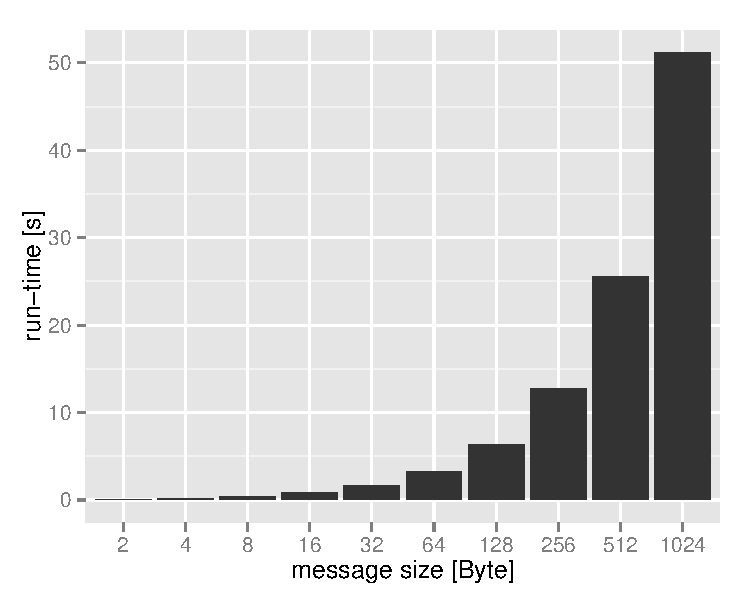
\includegraphics[width=.5\linewidth]{figures/runtime}
%% \caption{Run-time of algorithm X on machine Y.}
%% \label{fig:runtime}
%% \end{figure}

%% \subsection{Evaluating the Space Requirements of Algorithm X}

%% Now, we investigate the space requirements of the algorithms listed in Table~\ref{tab:related_algorithms}.


\section{Summary}
We summary the contribution of the papers and this seminar paper.
